\documentclass[letterpaper,12pt]{article}
\pdfpagewidth 8.5in
\pdfpageheight 11in 
\usepackage{graphicx}
\title{cPath:  Administrator Guide}
\author{cPath Development Team}
\date{January 22, 2008}
\begin{document}

\maketitle

\tableofcontents

% Todo:  Add details re:  the PSI-MI to BioPAX Converter.  Pending release by Ben.

\section{About this Document}

This document describes how to build a local installation of cPath, administer cPath via the command line, import BioPAX and PSI-MI files, and deploy the cPath web application.  This document refers only to the latest version of cPath (Version 0.7 Beta, from April, 2007).  For questions regarding this document or questions regarding cPath installation in general, please send email to Ethan Cerami (cerami AT cbio.mskcc.org).

\section{Introduction to cPath}

cPath is an open source pathway database and software suite designed for systems biology research. The main features of cPath include:

\begin{itemize}

  \item built-in support for the Biological Pathways Exchange (BioPAX) and Proteomics Standards Initiative Molecular Interaction (PSI-MI) XML formats.

  \item built-in identifier mapping service for linking identical interactors and linking to external resources.

  \item configurable web interface for browsing and searching biological pathways.

  \item simple HTTP URL based XML web service.

\end{itemize}

cPath is currently being developed by the Computational Biology Center at Memorial Sloan-Kettering Cancer Center, and the University of Toronto.

\bigskip

For a complete description of cPath software, please refer to:

\begin{itemize}
\item Ethan G Cerami, Gary D Bader, Benjamin E Gross, and Chris Sander, \textbf{cPath: open source software for collecting, storing, and querying biological pathways} BMC Bioinformatics 2006, 7:497 [doi:10.1186/1471-2105-7-497]
http://www.biomedcentral.com/1471-2105/7/497/abstract.
\end{itemize}

\section{System Requirements}

cPath can be installed on Linux, Windows or Mac OS X.  To begin, you must install the following:

\begin{itemize}

\item Java 1.5:  Information available at:  http://java.sun.com/j2se/1.5.0/

\item MySQL: Information available at: http://www.mysql.com/.  cPath has been tested with MySQL 4.0, 4.1, and 5.0. 

\item Apache Tomcat Server, 4.1X or above: Information available at: \linebreak
http://jakarta.apache.org/tomcat/.  cPath has been tested with Tomcat 4.1 and Tomcat 5.0. 
 
\item Apache Ant 1.6 (or later): Apache Ant is a software tool for automating software build processes.  Information is available at: http://ant.apache.org/. 
 
\item Perl 5.0 (or later): Information available at: http://www.perl.org/. 

\end {itemize}

\section{cPath Installation:  Step-By-Step Instructions }

This section provides complete step-by-step instructions to building a local installation of cPath.

\subsection{Getting Started}

\subsubsection{Install required software}

If you have not already done so, install Java 1.5, MySQL, Apache Tomcat, Apache Ant and Perl locally. Once you have verified that the installations are working correctly, proceed to the next step. 

\subsubsection{Download a cPath Source Distribution}

The cPath source is currently available for download at: 

http://cbio.mskcc.org/\verb+dev_site+/cpath/source.html.

\bigskip

We currently provide two download options:

\begin{itemize}

\item the current stable release:  this is the current stable release (version 0.7), now used in production;  and

\item the nightly snapshot:  this is the latest source code from our CVS repository.  This contains the very latest features, but please use at your own risk.

\end{itemize}

Once you have downloaded a source distribution, unzip it, and place it anywhere on your hard drive.  

\subsubsection{Set a CPATH HOME Variable}

Next, you will need to set a \verb+CPATH_HOME+ environment variable. This variable must point to the cPath distribution that you obtained in the previous step.  If you are using Mac OS X or Linux, you can do so via the shell. For example, here is an excerpt from a \verb+.bash_login+ file:

\begin{verbatim}
# Set up CPATH_HOME Variable
export CPATH_HOME=/Users/cerami/dev/sander/cpath
\end{verbatim}

\subsubsection{Configure your settings via the build.properties file}

The root cpath directory contains a configuration file named build.properties.  Before proceeding, you must configure the the database user/password properties in build.properties to match your current MySQL installation.  For example, you must set db.user to an existing MySQL user, and this user must have the rights to create new tables.  If you are not sure how to set up new MySQL users, and you are eager to get started, try setting db.name=root and set the appropriate password.  
 
Here is an excerpt from build.properties:

\begin{verbatim}
# Application Name and Version
app.name=cpath
app.version=0.7

# Database Settings
db.name=cpath
db.user=tomcat
db.password=kitty
db.host=localhost 
\end{verbatim}

Complete instructions on adding new MySQL users is available online at:
\verb+http://www.mysql.com/doc/en/Adding_users.html+.

\subsubsection{Create the cPath Database in MySQL}

Next, create the cPath database and tables.  To do so, run the initDb.pl script in the bin directory. For example:

\begin{verbatim}
> cd bin
> ./initDb.pl

Using CPATH_HOME /Users/cerami/dev/sander/cpath
Script to Initialize cPath Database
===================================

Using Database Name:      cpath
Using Database Host:      localhost
Using Database User:      tomcat
Using Database Password:  kitty

! Running this command will delete all existing data !
Are you sure you wish to proceed (Type: YES):  YES
Importing MySQL File:  cpath.sql
Importing MySQL File:  seed.sql
Importing MySQL File:  reference.sql
Done.  cPath is now ready to go...
\end{verbatim}

\subsection{Building cPath from Source Code}

Once the cPath database is set up, the next step is to compile and build cPath from source code.

\subsubsection{Compile cPath from Source Code}

To compile cPath, move to the root cPath directory and type:

\begin{verbatim}
> ant
\end{verbatim}

\subsection{Deploying the cPath Web Application}

If you have successfully followed all the steps above, you will now have an instance of cPath without any data.  As the next step, you will probably want to import some data.  But, if you are eager to deploy the cPath web application, follow the steps below.

\subsubsection{Generate the cPath WAR File}  
\label{generate-war}

The cPath WAR (Web Application Archive) contains the complete contents of cPath, ready for deployment to Tomcat. To generate the war file, move to the root cPath directory and type:

\begin{verbatim}
> ant war
\end{verbatim}

\subsubsection{Deploy cpath.war to Tomcat}

To do so, simply copy the cpath WAR file from build/war to your Tomcat webapps directory. For example:
\begin{verbatim}
cp build/war/cpath_0.5.war+ ~/libraries/jakarta-tomcat-5.0.28/webapps/
\end{verbatim}

Copying your war file here will cause Tomcat to automatically load and start cPath.

\subsubsection{Verify installation}

Open a web browser, and go to: http://localhost:8080/cpath/. Verify that you can see the cPath Home Page.  See Figure \ref{default-installation}.

\begin{figure}
  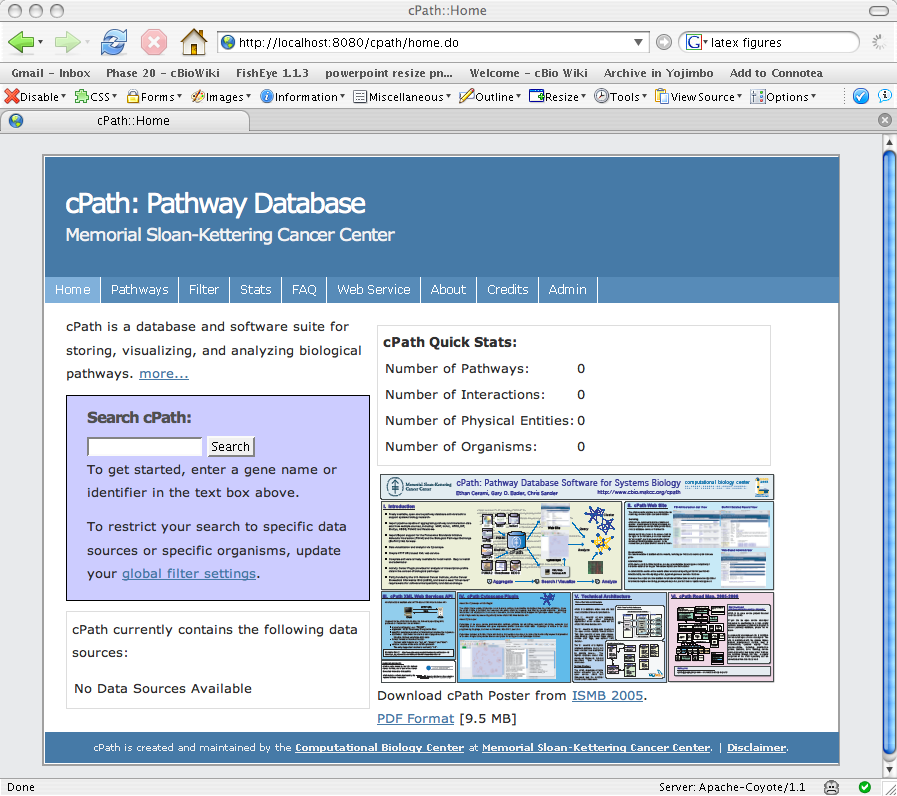
\includegraphics[scale=0.3]{figures/default_installation.png}
  \caption{Screenshot of the default cPath installation.}
\label{default-installation}
\end{figure}

\section{cPath Mode Options:  BioPAX v. PSI-MI}

\subsection{Description of cPath Mode Options}

cPath currently supports two mutually exclusive modes:  

\begin{itemize}

\item BioPAX mode: supports BioPAX files only.  However, in the near future, we will be releasing a command line tool for converting PSI-MI files to BioPAX, and this will enable users to integrate data from both formats into a single instance of cPath.  Note that the web service API for the BioPAX mode is not as extensive as in the PSI-MI mode, and there is no Cytoscape PlugIn for the BioPAX mode.  Both of these features represent active areas of development.  Future cPath development will focus on the BioPAX mode, but we plan to continue support for the PSI-MI mode for the foreseeable future.

\item PSI-MI mode: supports PSI-MI files only.  Provides an extensive web service API, and a Cytoscape cPath PlugIn for visualizing protein-protein interactions.

\end{itemize}

The most important decision regarding configuration will be your choice of mode.  If you want to import only PSI-MI protein-protein interactions, and query this data via a web service API or via the Cytoscape cPath plugin, you are best off choosing the PSI-MI mode.  If, on the other hand, you want to import BioPAX pathway records (or, in the future, a combination of BioPAX and PSI-MI records), you must choose the BioPAX mode.  The default cPath configuration is currently set to BioPAX mode.  If you wish to switch to PSI-MI mode, see section \ref{import-psi} below.

\section{Importing and Indexing BioPAX Data}

cPath currently supports BioPAX Levels 1 and 2.  Importing BioPAX data is a multi-step process: 

\begin{itemize}
\item First, load meta-deta regarding the source of your BioPAX data.  This includes information such as the database name, a database description, a database icon, etc.  This information is not currently available in BioPAX and requires that you create a separate XML file.

\item Second, create a small text configuration file for all the BioPAX files within a directory.  This configuration file ties all the BioPAX files within a single directory to a specific release number/version of a specific database.

\item Third, import your BioPAX files.

\item Fourth, run the PubMed fetcher command to look-up all missing PubMed details.  This command connects to NCBI and automatically downloads any missing titles, authors, or citation information for all PubMed IDs.

\item Fifth, run the index command.  This indexes all the BioPAX records, and enables all search functionality.

\item Finally, regenerate the cPath WAR file, and deploy the cPath web application.

\end{itemize}

Complete details regarding each step is provided below.

\subsection{Import Database Meta-Data Details}

The first step is to load meta-data regarding the source of your pathway data.  This meta-data contains details about the source database, including the name of the database, a short description, home page URL, etc.  For example, if you are loading a BioPAX file from Reactome, you must first load meta-data regarding Reactome into cPath.  The meta-data is very important, as it provides a means to link back to the original data provider, and give them due credit.

To create a meta-data file, you must first create a valid XML configuration file, and then explicitly load this file into cPath.  A sample meta-data file is found in \verb+dbData/externalDb/pathway_commons.xml+.  This file loads all meta-data for all sources currently found at pathwaycommons.org.

Below is an excerpt:

\begin{verbatim}
<?xml version="1.0" encoding="UTF-8"?>
<!DOCTYPE external_database_list SYSTEM "external_db.dtd">
<external_database_list>
    <external_database type="INTERACTION_PATHWAY_UNIFICATION">
        <name>Reactome</name>
        <description>Reactome: a knowledgebase of...</description>
        <home_page_url>http://reactome.org</home_page_url>
        <entity_url>
            <url_pattern>http://reactome.org/cgi-bin/...</url_pattern>
            <sample_id>12345</sample_id>
        </entity_url>
        <icon_path>Reactome.png</icon_path>
        <controlled_terms>
            <master_term>REACTOME</master_term>
        </controlled_terms>
    </external_database>
    ...
\end{verbatim}

Using this as a sample, you can probably figure out how to create your own meta-data configuration files.  Note that you can also include a database icon by specifying the \verb+icon_path+ element.  For best results, database icons should be approximately 66 x 66 pixels large.

Once you have created a meta-data file, move to \verb+[CPATH_HOME]\bin+, and load the file via the admin.pl script.  For example:

\begin{verbatim}
> cd bin
> ./admin.pl -f ../dbData/externalDb/pathway_commons.xml import
\end{verbatim}

In the example above, the -f flag specifies the location of the meta-data file, and the import command indicates that you wish to import new data.

\subsection{Create a db.info configuration file}

For simplicity, all the BioPAX files within a single directory must originate from the same data source.  This data source information is specified in a small db.info text configuration file.  A sample db.info file is found in \verb+testData/biopax/db.info+.  Below, are the complete contents of this file:

\begin{verbatim}
# Sample db.info
# this file is required for loading BioPAX data from this directory
db_name=Reactome
db_snapshot_version=1.0
db_snapshot_date=01/02/2006
\end{verbatim}

Note that the \verb+db_name+ field must match a database name element from one of your meta-data XML files (see above).  Note also, that if you do not have version or date information, you can simply specify the text, ``N/A''.

\subsection{Import BioPAX Files}

Next, import your BioPAX files.  For example, the following command loads the Reactome Apoptosis pathway:

\begin{verbatim}
> cd bin
> ./admin.pl -f ../testData/biopax/Apoptosis.owl import
\end{verbatim}

If you have neglected to create a db.info file in the same directory as your BioPAX file, you will receive an error message.

\subsection{Fetch PubMed Details}

Once you have imported all your BioPAX files, the next step is to run the PubMed Fetcher.  If a BioPAX record contains a PubMed ID, but does not contain the complete citation information regarding the article, the fetcher will automatically retrieve this data from PubMed.  To run the fetcher, type:

\begin{verbatim}
> cd bin
> ./admin.pl pop_ref
\end{verbatim}

Note that cPath honors the NCBI request to include a 3 second delay between batch requests.  So, downloading all PubMed records may take some time.

\subsection{Index BioPAX Records}

Finally, to enable the cPath search engine, you must index all cPath records and create a full-text index.  To do so, run the index command.  For example:

\begin{verbatim}
> cd bin
> ./admin.pl index
\end{verbatim}

Remember to re-index cPath after importing any new data.

\subsection{Regenerate the WAR File}

Once all your data has been imported and indexed, you must re-generate the WAR file and redeploy to Tomcat.  See \ref{generate-war} above.

\section{Importing and Indexing PSI-MI Data}
\label{import-psi}

cPath currently only supports the importing of PSI-MI Level 1 files.  It does not support PSI-MI Level 2.5.  Importing PSI-MI data is considerably simpler than importing BioPAX files, and requires only four steps.

\begin{itemize}
\item First, import your PSI-MI files.

\item Second, run the index command.  This indexes all the PSI-MI records, which is required for search.

\item Third, set cPath to PSI-MI mode.

\item Finally, regenerate the cPath WAR file, and deploy the cPath web application.

\end{itemize}

Complete details regarding each step is provided below.

\subsection{Import PSI-MI Records}

First, import your PSI-MI files.  For example, the following command loads a sample PSI-MI file from DIP (Database of Interacting Proteins):

\begin{verbatim}
> cd bin
> ./admin.pl -f ../testData/psi_mi/dip_psi.xml
\end{verbatim}

\subsection{Index PSI-MI Records}

To enable the cPath search engine, you must index all cPath records and create a full-text index.  To do so, run the index command.  For example:

\begin{verbatim}
> cd bin
> ./admin.pl index
\end{verbatim}

Remember to re-index cPath after importing any new data.

\subsection{Set cPath to PSI-MI Mode}

By default, the cPath web application is set to the BioPAX mode.  To set cPath to the PSI-MI mode, you must modify the web.skin property in build.properties.  Below is an example:

\begin{verbatim}
# Skin:  default_psi_mi, default_biopax, pathwaycommons, etc.
web.skin=default_psi_mi
\end{verbatim} 

\subsection{Regenerate the WAR File}

Once you have configured build.properties, and all your data has been imported and indexed, you must re-generate the WAR file and redeploy to Tomcat.  See \ref{generate-war} above.

\section{Importing Identifier Mapping Files}

A recurring problem in bioinformatics is linking related or identical data described by different databases when multiple database identifiers (primary keys) are used to refer
to the same biological entity. Interaction databases may use different identifiers for their proteins, RNA, DNA or small molecules (for example, a protein may be identified with a UniProt accession number, RefSeq accession number or an NCBI GI number). This use of multiple
identifiers can significantly hinder the ability to seamlessly use data from diverse sources, such as to retrieve all interactions involving a protein from numerous data sources. Recognizing when protein records that use different database identifiers actually represent the same protein allows a query for the protein to correctly retrieve both original records. To address this specific issue, cPath provides an identifier mapping system capable of
storing equivalence between two or more identifiers. 

For example, a single protein unification mapping may map UniProt accession numbers to equivalent RefSeq accession numbers. Identifier mapping files are simple tab-delimited text files that must be loaded into cPath prior to import of any interaction or pathway data sets. With some scripting ability, cPath identifier mapping files can be created from external database resources, such as Alias Server, the EBI International Protein Index (IPI), or Ensembl BioMart. Sample protein unification files, derived from the IPI Protein Cross-References dataset, are available in \verb+CPATH_HOME/scripts+.

For example, below is an excerpt from the \verb+cpath_unification_sp2refseq.txt+ file.  This file maps UniProt IDs to RefSeq IDs:

\begin{verbatim}
UNIPROT REF_SEQ Protein
O03042  NP_051067
O03983  NP_171654
O04005  NP_175247
O04027  NP_172377
O04036  NP_001031006
O04036  NP_001031006
O04046  NP_179960
O04090  NP_172565
O04093  NP_172561
\end{verbatim}

To import an ID mapping file, use the admin.pl command line tool.  For example:

\begin{verbatim}
./admin.pl -f ../scripts/cpath_unification_sp2refseq.txt import
\end{verbatim}

A script for automatically downloading the latest IPI data and creating ID mapping files is available in \verb+CPATH_HOME/scripts/parse_ipi-2.pl+.  For question regarding the IPI script, please contact Ruth Isserlin at the University of Toronto (ruth.isserlin AT utoronto.ca).

Importantly, cPath also provides a similar service for storing relationships between non-equivalent, but related biological entities. For example, a researcher can import a
UniProt to Affymetrix mapping file.  When a new protein with a matching UniProt identifier is subsequently imported into cPath, it is annotated with all known Affymetrix probe set identifiers. This is useful for tools that link gene expression data to pathways.

A sample link-out ID mapping file that maps Affymetrix \verb+HG_U95+ probeset IDs to UniProt/SwissProt IDs to is provided in \verb+CPATH_HOME/testData/affymetrix/HG_U95Av2.txt+.  

\section{Troubleshooting cPath}

If you experience problems with the cPath web application, here are a few things to try out.

\subsection{Running cPath Diagnostics}

In the event of an error, the first place to check is the cPath Diagnostics page:

\begin{itemize}

\item Go to:  \verb+http://localhost:8080/cpath/adminHome.do+

\item Enter the admin user name and password.  This is specified in build.properties, and the default settings are:  user=admin, password=cpath.

\item Click the link, labeled ``Run cPath Diagnostics''.

\end{itemize}

This page tests access to all the cPath tables and to the cPath full-text indexer.  If everything is set-up correctly, you should see a series of green check arrows (See Figure \ref{cpath-diagnostics}). Failures are noted in red.  

\begin{figure}
  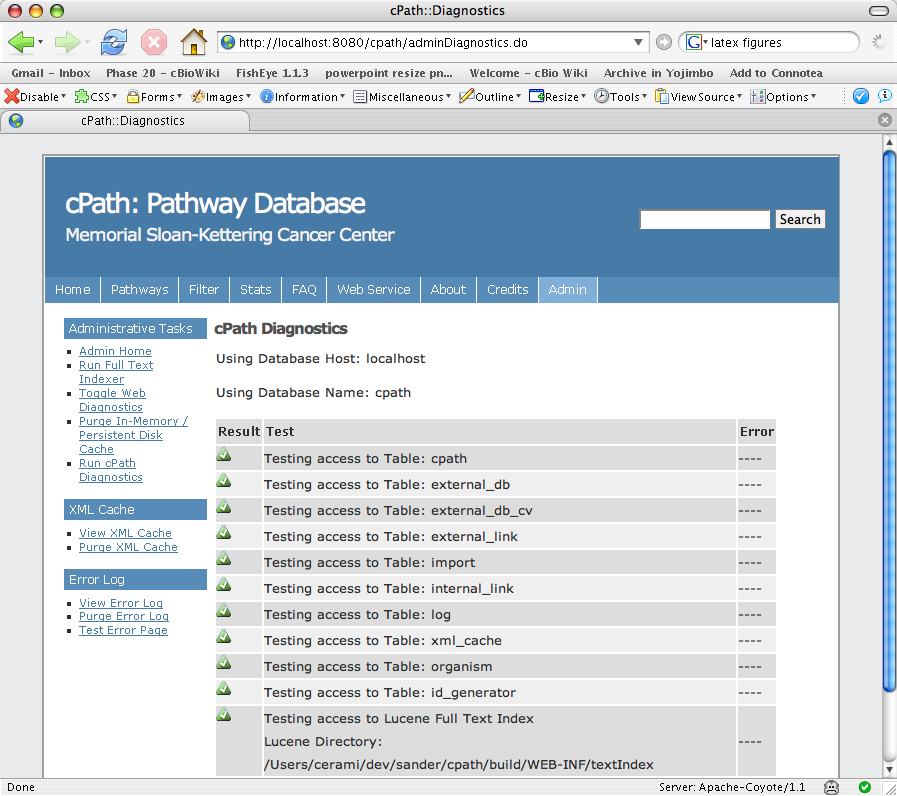
\includegraphics[scale=0.3]{figures/cpath_diagnostics.png}
  \caption{Screenshot of the cPath diagnostics page.}
\label{cpath-diagnostics}
\end{figure}

\subsection{Clearing the In-memory / Persistent cache}
\label{purge-cache}

cPath uses an in-memory / persistent disk cache.  The cache is persistent across restarts of cPath or of Apache tomcat.  Occasionally, you may encounter strange behavior like the following:

\begin{itemize}

\item First, you load up some data, and deploy the cPath web application.

\item You then go to the home page and view the database statistics.

\item You then load up some more data and recheck the database statistics.  However, you notice that the database statistics have not been updated.

\item You then try to restart Apache tomcat, and the statistics are still not updated!  What is going  on?

\end{itemize}

This scenario occurs because the database statistics (plus lots of other components, including search results) are cached (first in memory, and then on disk).  We do this to optimize the performance of the web application, but as noted above, it can lead to some puzzling results.

To solve the problem, you must manually clear the cache via the cPath web administrator page.

\begin{itemize}

\item Go to:  \verb+http://localhost:8080/cpath/adminHome.do+

\item Enter the admin user name and password.  This is specified in build.properties, and the default settings are:  user=admin, password=cpath.

\item Click the link, labeled ``Purge In-Memory / Persistent Disk Cache''.

\item Also, click the link, labeled ``Purge XML Cache''.

\end{itemize}

As a rule, you should purge the cache every time you either 1) import or index new data;  or 2)  make a change to build.properties.

\subsection{Tracking Down Errors with Web Diagnostics}

Occasionally, you will receive a web page error.  If you want to view live web diagnostic information, simply append a debug=1 parameter at the end of any cPath URL.

For example, this URL activates web diagnostics for the cPath home page (See \ref{web_diagnostics}). 

\begin{verbatim}
http://localhost:8080/cpath/adminHome.do?debug=1
\end{verbatim}

\begin{figure}
  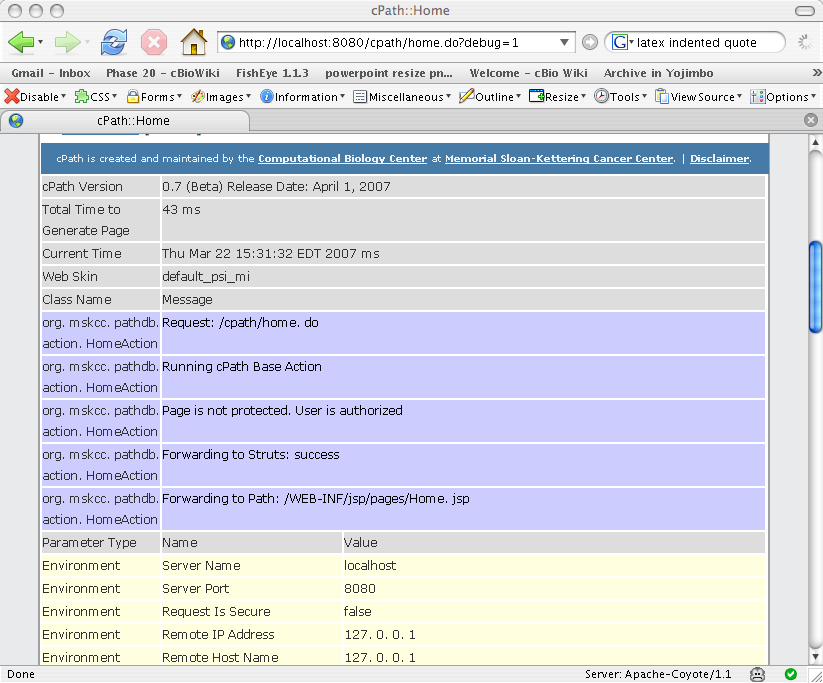
\includegraphics[scale=0.3]{figures/web_diagnostics.png}
  \caption{Screenshot of the cPath web diagnostics in action.}
\label{web_diagnostics}
\end{figure}

You can try this on any cPath page, and you will immediately view many details, including:

\begin{itemize}

\item A detailed stack trace (if an error has occurred).

\item Environment and servlet variables.

\item Logging messages.

\item Client / Server details, including the remote host and IP address.

\item All HTTP Headers.

\item Session and Cookie details.

\end{itemize}

You also have the option of activating / de-activating web diagnostics for all cPath pages.  To do so:

\begin{itemize}

\item Go to:  \verb+http://localhost:8080/cpath/adminHome.do+

\item Enter the admin user name and password.  This is specified in build.properties, and the default settings are:  user=admin, password=cpath.

\item Click the link, labeled ``Toggle Web Diagnostics''.

\end{itemize}

\subsection{Starting Over with an Empty Database}

If you want to start over with a fresh/empty cPath database, simply run initDb.pl:

\begin{verbatim}
> cd bin
> ./initDb.pl
\end{verbatim}

Note that this will delete all existing data.

\section{Configuring cPath}

\subsection{Configuring web skins}

cPath currently supports three web skins:

\begin{itemize}

\item \verb+default_biopax+:  Default BioPAX Web Skin (the default setting).

\item \verb+default_psi_mi+:  Default PSI-MI Web Skin.

\item pathwaycommons:  Web Skin currently used by PathwayCommons.org.
\end{itemize}

To configure your web skin, simply modify build.properties.  For example:

\begin{verbatim}
# Skin:  default_psi_mi, default_biopax, pathwaycommons, etc.
web.skin=pathwaycommons
\end{verbatim}

Then:

\begin{itemize}

\item Regenerate the cPath WAR file, and deploy the cPath web application.

\item Remember to purge the in-memory / disk cache each time you tweak your build.properties file (see

\ref{purge-cache} above).
\end{itemize}

\subsection{Creating new web skins}

\subsubsection{Overview}
If you know some HTML and a bit of Java Server Pages (JSP), you can create new web skins to match your local installation of cPath.  For example, you can customize the following web components:

\begin{itemize}

\item Header and logo.

\item Footer.

\item Complete contents of the home page.

\item The ``About'' page describing your local installation.

\item The ``FAQ'' page describing your local installation.

\end{itemize}

\subsubsection{To create new web skin}

\begin{itemize}

\item Create new directory under \verb+web/WEB-INF/jsp/skins+.  For example, create a new directory called, \verb+my_skin+.

\item If you are creating a new PSI-MI web skin, copy all the .jsp files in \verb+web/WEB-INF/jsp/skins/default_psi_mi+ to your new directory.

\item If you are creating a new BioPAX web skin, copy all the .jsp files in \verb+web/WEB-INF/jsp/skins/default_biopax+ to your new directory.

\item Using the newly copied JSP files as templates, create your own skin.  For example, to modify the header, modify the HTML in your new header.jsp file.

\item Modify your build.properties file to point to your new web skin.  For example:

\begin{verbatim}
# Skin:  default_psi_mi, default_biopax, pathwaycommons, etc.
web.skin=my_skin
\end{verbatim}

\item Regenerate the cPath WAR file, and deploy the cPath web application.

\item Remember to purge the in-memory / disk cache each time you tweak your JSP files (see

\ref{purge-cache} above).
\end{itemize}

\subsection{Configuring the Cytoscape cPath PlugIn}

The Cytoscape cPath Plugin (now available in Cytoscape 2.4) can connect to any instance of cPath in PSI-MI mode.  To configure the Cytoscape cPath PlugIn to point to a local installation of cPath:

\begin{itemize}
\item Start Cytoscape.

\item From the main Cytoscape menu, select:  Edit::Preferences::Properties.

\item Click ``add'' new property.

\item Set property name to:  \verb+cpath.url+.

\item Set value to, e.g.:  \verb+http://localhost:8080/cpath/webservice.do+.

\item If you want this property to persist in all future Cytoscape settings, click the checkbox for:  ``Make Current Cytoscape Properties Default''.
\end{itemize}

\subsection{Taking cPath Offline}

If you are running a production version of cPath, and need to do some type of maintenance, e.g. load new data, you can temporarily take the entire cPath site offline:

\begin{itemize}

\item Go to:  \verb+http://localhost:8080/cpath/adminHome.do+.

\item Enter the admin user name and password.  This is specified in build.properties, and the default settings are:  user=admin, password=cpath.

\item Click the link, labeled ``Take Site Offline''.
\end{itemize}

When offline, the cPath home page will display the following message: ``cPath is currently down for a scheduled upgrade. Please check back in approximately 30 minutes.''

\section{Known Issues}

\subsection{Known Issue: Packet Too Big Exception}

\subsubsection{Symptoms}  

You attempt to import a very large data file, and receive the following error message: PacketTooBigException.

\subsubsection{Diagnosis} 
This error occurs because cPath stores the complete contents of all imported records in the MySQL database.  If the imported record exceeds the MySQL \verb+max_allowed_packet+ setting, you will receive a PacketTooBigException.

\subsubsection{Solution}
To fix this problem, increase the MySQL setting for \verb+max_allowed_packet+.

The simplest way to do so is to update (or create) a my.cnf configuration file.  For example, the following file (/etc/my.cnf) increases the \verb+max_allowed_packet+ to 65M:

\begin{verbatim}
[mysqld]
max_allowed_packet=65M
\end{verbatim}

\subsubsection{Resources}

\begin{itemize}

\item Complete details regarding the ``Packet too Large'' issue is available at:  \verb+http://dev.mysql.com/doc/mysql/en/Packet_too_large.html+.

\item Complete details regarding “Using Option Files”, and configuring MySQL settings, see: \verb+http://dev.mysql.com/doc/mysql/en/Option_files.html+.

\end{itemize}

\subsection{Known Issue: Out of Memory Error}

\subsubsection{Symptoms}
You attempt to import a very large data file and receive the following error message: OutOfMemoryError.

\subsubsection{Diagnosis}
This error occurs because cPath stores the complete contents of a single imported record in memory before writing to the MySQL database.

\subsubsection{Solution}
To fix this problem, increase the memory available to Java.   To do so, simply increase the \verb+-Xmx+ value in \verb+bin/admin.pl+.

\section{Appendix A: Monitoring cPath for Constant Uptime}

Once installed, it is useful to monitor cPath on a periodic basis, and verify that it is running correctly. A recommended tool is TinyMonitor, available from: http://www.glug.com/projects/TinyMonitor/. From the Glug.com site:

\begin{quote}
TinyMonitor was written out of pure necessity for a simple monitoring program that watched the actual content of returned pages rather than simply checking to see if the httpd service was running. (Experience has proven that the web server running doesn't necessarily mean it's reporting the content you want.)

This program can be used for simple web server monitoring (i.e. is it actually delivering content?) or can be used to verify a page is returning what you expect (i.e. a 200 rather than a 404). This is an excellent choice for someone who doesn't want to spend thousands on a program that will do actual http content monitoring (i.e. SiteScope or HP OpenView Internet Services).
\end{quote}

A copy of TinyMonitor (along with a sample config file for monitoring cPath) is available in bin/tinymonitor.

\end{document}             % End of document.
